\documentclass{article}
\usepackage{amsmath}
\usepackage{graphicx}
\usepackage{tikz}
\usepackage{pifont}
\usepackage[fontsize=14pt]{fontsize}

\title{Negative Numbers\\\& Real Numbers\\Course\\
\begin{center}

\includegraphics[width=4em]{ApS_logo.png}
\end{center}
\begin{normalsize}Tutoring Centre Ferndale \end{normalsize}}
\author{}
\date{}

\begin{document}
\maketitle

\section*{Negative numbers}

\paragraph{Negative}
Negative means denial or saying no to something, or being on the opposite side to something, as in "the covid test result was negative" or "the bosses answer was negative so we couldn't do it."

\begin{enumerate}

\item What does negative mean, in your own words?
\item Use negative in 5 sentences.

\paragraph{Positive}
Positive means definite and existing, or saying yes to something, as in "he was positive that he could do it" or "the covid test was positive."

\item What does positive mean, in your own words?
\item Use positive in 5 sentences.

\begin{center}
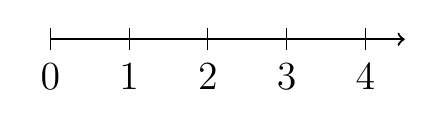
\begin{tikzpicture}
	\draw [->,thick](0,0) -- (4.5,0);
	\foreach \x in {0,...,4}
	\draw (\x,4pt) -- +(0,-8pt) node [below] {$\x$};
\end{tikzpicture}
\end{center}

\paragraph{Positive Numbers}
Numbers to the right of 0 on a number line are called positive numbers. They represent amounts that do exist and can be counted.

Positive numbers are indicated by a $+$ sign to the left of the number, but that is not normally written because numbers are assumed to be positive numbers.

\item What is a positive number, in your own words?
\item How would you mark a number to make it clear that you mean it to be a positive number?

\paragraph{Negative Numbers}
Numbers can exist that are less than 0. They are different to the sort of numbers that are used for counting real things. They are called negative numbers and they are on the opposite side of the number line to positive numbers.

Negative numbers are written by putting a minus sign to the left of the number. "$-5$" is read as "negative five."\\

Subtraction of a smaller number from a larger number, such as $3-2=1$, can be shown by moving to the left on a number line.\\

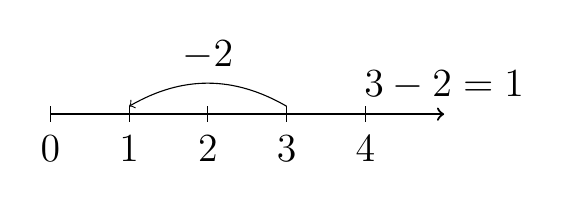
\begin{tikzpicture}
\draw[thick, ->] (0,0) -- (5,0) node[above] {$3-2=1$};
\foreach \n in {0,1,2,3,4} {\draw (\n,0.1) -- (\n,-0.1) node[below] {$\n$};}
\draw[->, bend right=30] (3,0.1) to node[above] {$-2$} (1,0.1);
\end{tikzpicture}

Negative numbers can be visualised by extending a number line to the left of 0.\\

\begin{center}
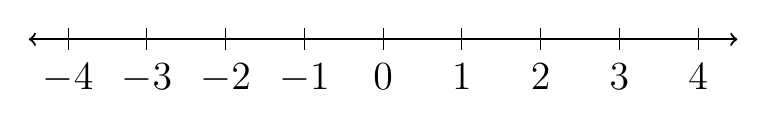
\begin{tikzpicture}
	\draw [<->,thick](-4.5,0) -- (4.5,0);
	\foreach \x in {-4,...,4}
	\draw (\x,4pt) -- +(0,-8pt) node [below] {$\x$};
\end{tikzpicture}
\end{center}

You come across negative numbers when subtracting a larger number from a smaller number.\\

Say you have 3 of something \ding{46}\ding{46}\ding{46} and someone wants 5 of them \ding{46}\ding{46}\ding{46}\ding{46}\ding{46} there are still 2 more needed. \ding{46}\ding{46}\\

As an equation, that is $3-5=-2$. On a number line that extends to the left with numbers less than 0, this looks like:

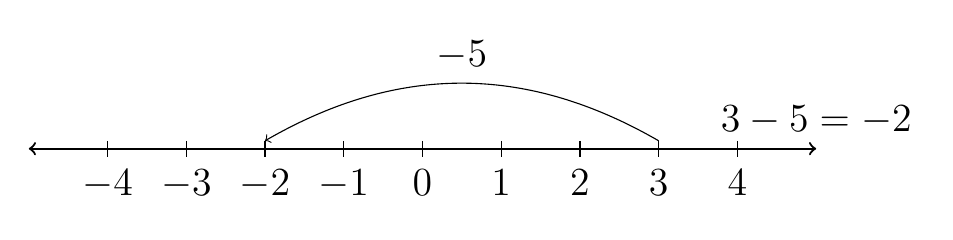
\begin{tikzpicture}
\draw[thick, <->] (-5,0) -- (5,0) node[above] {$3-5=-2$};
\foreach \n in {-4,-3,-2,-1,0,1,2,3,4} {\draw (\n,0.1) -- (\n,-0.1) node[below] {$\n$};}
\draw[->, bend right=30] (3,0.1) to node[above] {$-5$} (-2,0.1);
\end{tikzpicture}

 With negative numbers the difference between any two numbers can be found, even when the answer is less than 0.\\

 You can also think of negative numbers as, instead of having some amount of things, those things are owed as a debt.

\item What is a negative number, in your own words?
\item Use negative number in a sentence.
\item How are negative numbers written?

\paragraph{Directed Numbers}
Numbers that can be either negative or positive are known as directed numbers. They have a value and they also have a direction either above or below 0. Examples of directed numbers are temperature, which can be above or below 0 degrees, and altitude, which is above or below sea level.

\item What are directed numbers, in your own words?
\item What is another example of a directed number?

\subsection*{Integers} 
All of the natural numbers plus all of the negative numbers, and zero, are called integers. Integer means ‘untouched,’ meaning that it is a whole amount that hasn't been broken into smaller parts. Fractions, whether positive or negative, are not integers.

\item What are integers?
\item Use integer in a sentence.
\item Write any 5 integers.

\section*{Addition\\ with Negative Numbers}

Adding a negative number to a positive number is the same as subtracting the negative number.

$$5+(-3)=2 \textrm{ is the same as } 5-3=2.$$
$$5+(-8)=-3 \textrm{ is the same as } 5-8=-3.$$

Negative numbers are enclosed in brackets like this when they are written next to other numbers or symbols that could cause confusion.

\item What is $3+(-2)$?
\item What is $-3+5$?
\item What is $12+(-8)$?
\item What is $-15+6$?
\item What is $-8+9$?

\section*{Subtraction\\ with Negative Numbers}

Subtracting a negative number from any other number is the same as adding the negative number.

Say a bank had charged you \$10 by mistake and then took away the \$10 charge. That negative amount has been subtracted, so you now have \$10 more than you did before.

$$5-(-3)=8 \textrm{ is the same as } 5+3=8.$$
$$(-5)-(-8)=3 \textrm{ is the same as } -5+8=3.$$

\item What is $3-(-2)$?
\item What is $-3-5$?
\item What is $12-(-8)$?
\item What is $-15-6$?
\item What is $-8-9$?

\section*{Multiplication\\ with Negative Numbers}

Multiplying a positive number by a negative number gives a negative product.
$$5\times(-3)=-15.$$

Borrowing \$5 3 times means you now owe \$15.

Multiplying a negative number by another negative number gives a positive product.
$$(-5)\times(-3)=15.$$

If you owed \$5 to 3 people and they all said to forget it and keep your money then you have gained \$15.

\item What is $3\times-2$?
\item What is $-3\times-5$?
\item What is $12\times-8$?
\item What is $-15\times6$?
\item What is $-8\times9$?

\section*{Division\\ with Negative Numbers}

Dividing a positive number by a negative number, or dividing a negative number by a positive number, both give a negative quotient.
$$15\div(-3)=-5.$$
$$-15\div3=-5.$$

If 3 people wanted an equal share of your \$15 then you would owe each of them \$5.

Dividing a negative number by another negative number gives a positive quotient.
$$(-15)\div(-3)=5.$$

To owe \$15 you borrowed \$3 from 5 people.

\item What is $8\div-2$?
\item What is $-15\div5$?
\item What is $12\div-8$?
\item What is $-15\div-3$?
\item What is $-8\div-4$?

\section*{Real numbers}

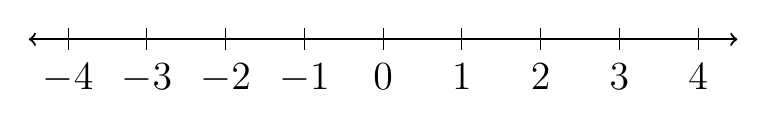
\begin{tikzpicture}
\draw [<->,thick](-4.5,0) -- (4.5,0);
\foreach \x in {-4,...,4}
\draw (\x,4pt) -- +(0,-8pt) node [below] {$\x$};
\end{tikzpicture}\\

Integers can be represented as specially-marked points evenly spaced on a number line, but that is only the whole numbers. Real numbers are at every point on the line, not just at the points of the integers. Amounts that change continually, such as temperature or distance, are real numbers.\\

\begin{tikzpicture}
\draw [<->,thick](-4.5,0) -- (4.5,0);
\foreach \x in {-4,...,4}
\draw (\x,4pt) -- +(0,-8pt) node [below] {$\x$};
\draw [<-] (-2.5,-0.05) -- (-2.5,-2) node [below] {$-2\frac{1}{2}$};
\draw [<-] (3.142857,-0.05) -- (3.142857,-2) node [below] {$\frac{22}7}$};
\draw [<-] (0.75,-0.05) -- (0.75,-2) node [below] {$\frac{3}{4}$};
\draw [<-] (1.72,-0.05) -- (1.72,-2) node [below] {$1.72$};
\end{tikzpicture}\\

\item What are real numbers, in your own words?
\item Use real numbers in a sentence.
\item Write 5 examples of real numbers.

\paragraph{Infinity}

Something that is finite has an end somewhere. Infinity, something that is infinite, is endless.

The symbol for infinity is "$\infty.$"

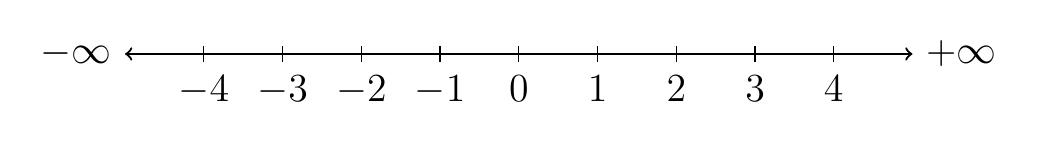
\begin{tikzpicture}
\draw[<->,thick] (-5,0) -- (5,0);
\node[left] at (-5,0) {$-\infty$};
\node[right] at (5,0) {$+\infty$};
\foreach \x in {-4,...,4}
\draw (\x,0.1) -- (\x,-0.1) node[below] {$\x$};
\end{tikzpicture}

The number line goes on forever in both directions without ending, towards infinity.

Infinity is the idea that no matter how big the number is that you think of, whether positive or negative, there can always be an even bigger number.

Infinity isn't actually a number. Things in the real world can only go towards infinity. They can't ever reach it.

\item What does finite mean, in your own words?
\item Use finite in a sentence.
\item What does infinite mean, in your own words?
\item Use infinite in a sentence.
\item What is infinity, in your own words?
\item Use infinity in a sentence.

\subsection*{Rational Numbers}

A ratio is an amount of one thing compared to an amount of some other thing. A "3 to 4" ratio means that there are 3 of something for every 4 of something else. A ratio can also be expressed as a fraction. For a 3 to 4 ratio, $\frac{3}{4}$ of the total amount must be something and $\frac{1}{4}$ of it must make up the rest.\\

\item What is a ratio?
\item Use ratio in a sentence.
\item Think of a ratio, and write it both as a ratio and as a fraction.

Rational means to do with ratios, and it also means something that makes sense or is logical.

\item What are the two meanings of rational?
\item Use rational in a sentence for each of these meanings.

If a number can be expressed exactly as a ratio of two numbers, such as $\frac{3}{4}$ or $\frac{-6}{5}$, then it is called a rational number.\\

Integers and whole numbers are rational numbers as well because they can all be expressed as a ratio of themselves to one, such as $3=\frac{3}{1}$ or $-27=\frac{-27}{1}$.\\

\item What is a rational number?
\item Use rational number in a sentence.
\item Write an example of a rational number.
\item Is $\frac{2}{3}$ a rational number? Why?
\item Is 5 a rational number? Why?

\subsection*{Irrational Numbers}

Irrational means not reasonable, and it means something that can't be written as a ratio.

\item What are the two meanings of irrational?
\item Use irrational in a sentence for each of these meanings.

Real numbers that can't be written as a ratio of two other numbers are called irrational numbers.\\

Irrational numbers can be precisely defined, such as "the number which when multiplied by itself has a product of 2," but they are not a ratio of any two numbers, and the digits of an irrational number written as a decimal fraction would go on forever.\\

\item What is an irrational number, in your own words?
\item Use irrational number in a sentence.

\subsubsection*{\Large{$\pi$} Pi}
Perimeter means the length around the outside of a shape.
\item What does perimeter mean, in your own words?
\item Use perimeter in a sentence.

Circumference means the length around the outside of a circle.
\item What does circumference mean, in your own words?
\item Use circumference in a sentence.

Diameter means the length across the middle of a circle.
\item What does diameter mean, in your own words?
\item Use diameter in a sentence.

The Greek letter $\pi$ (pi) stands for "perimeter" and represents the ratio of the circumference to the diameter of a circle.

$\Large{\pi} = \frac{\text{circumference}}{\text{diameter}}\approx3.14159\dots$ is a well-known irrational number that is used in all sorts of problems involving circles. Calculating $\pi$ as a decimal fraction is used as a test for computing power and has been done to trillions of digits so far. People have also memorized the digits of $\pi$ to tens of thousands of digits.

\item What does $\pi$ mean, in your own words?
\item Use $\pi$ in a sentence.

\subsubsection*{Terminating and Non-Terminating\\Decimal Fractions}

The digits in a decimal fraction will either terminate at some point, such as 3.752, or a digits will repeat itself endlessly, such as in $\frac{1}{9}=0.1111\dots$, or a sequence of numbers will start to repeat endlessly, such as in $\frac{22}{7}=3.142857142857\dots$, or digits will go on forever without repeating, as in the value of $\pi = 3.14159\dots$. Decimal fractions that do not repeat or terminate are irrational numbers.\\

An endlessly repeating digit of a decimal fraction is marked by putting a dot above that digit, such as $\frac{1}{3}=0.33\ldots=0.\dot{3}.$\\

An endlessly repeating series of digits such as in $\frac{22}{7}=3.142857142857142857\dots$ is written as $3.\overline{142857}$ with a line drawn over the repeating part of the decimal.\\

\item What is a terminating decimal fraction?
\item Give an example of a terminating decimal fraction.

\item What is a repeating decimal fraction?
\item Write an example of a decimal fraction where one digit repeats endlessly.
\item Write an example of a decimal fraction where a series of digits repeats endlessly.

\item What is a non-terminating non-repeating decimal fraction?
\item Give an example of a decimal fraction that does not terminate and does not repeat.
\item Is a non-terminating non-repeating decimal fraction a rational number or an irrational number?

\subsubsection*{Converting a Repeating\\Decimal Fraction\\into a Fraction}

Every rational number can be written as either a repeating or terminating decimal fraction.

Using algebra, all repeating decimal fractions can be converted to exact fractions or ratios.

Create an equation setting the repeating decimal fraction  equal to $x$. Multiply that equation by a power of 10 so that the repeating part of the fraction is shifted to the left of the decimal point. Subtract the two equations.

\begin{align}
                            x&=0.\overdot{7}\\
\text{(1) $\times 10$ : } 10x&=7.\overdot{7}\\
      \text{(2) - (1) : }  9x&=7\\
                            x&=\frac{7}{9}
\end{align}

\setcounter{equation}{0}

\begin{align}
x&=0.\overline{24}\\
\text{(1) $\times 100$ : }
100x&=24.\overline{24}\\
\text{(2) - (1) : }
\ 99x&=24\\
x&=\frac{24}{99}=\frac{8}{33}
\end{align}

\item Convert the repeating decimal $0.\dot{3}$ to a fraction.
\item Express $0.\overline{625}$ as a fraction.
\item Convert $1.\dot{2}$ to a fraction.

\end{enumerate}

\end{document}
